\chapter{Projektumsetzung}
In dem einjährigen Projekt der Projektgruppe Routing in Oldenburg gibt es verschiedene Phasen in der Erarbeitung und Umsetzung der Projektziele.
Die Projektumsetzung unterteilt sich grundsätzlich in zwei verschiedene Phasen.
Zum einen die Vorbereitungsphase, in denen Dinge wie ein Visionsdokument, ein Anforderungsdokument, die Architektur der Softwarekomponenten und Ähnliches erarbeitet werden.
Zum anderen gibt es die anschließende Umsetzungsphase (auch Implementierungs- oder Entwicklungsphase), in der die erarbeiteten Dokumente aus der Vorbereitungsphase genutzt werden, um die Software auf Basis mehrerer Meilensteine zu implementieren.
Das Ziel eines jeden Meilensteins ist es dabei, die Software nach dem grundsätzlichen Setup und dem technischen Durchstich, um Features zu erweitern, welche soweit wie möglich zwischen den einzelnen Komponenten abgestimmt sind.
So soll mit jedem Meilenstein das Produkt um ein in sich sinnvolles und vollständiges Paket beziehungsweise Release erweitert werden.
Dabei muss berücksichtigt werden, dass die Arbeitsweise der Projektgruppe auf dem agilen Vorgehensmodell SCRUM beruht.
Es wird also agil mit Anfoderungen und Projektumsetzung umgegangen (siehe dazu Dokumentation Teil III, Abschnitt 1.7)

In den folgenden Kapiteln soll der Fokus auf die praktische Umsetzung der einzelnen Softwarekomponenten gelegt werden.
Hierzu wird beschrieben, wie die Implementierungsphase gegliedert ist, auf welche Aspekte zu welchem Zeitpunkt besonderen Wert gelegt wird und welche Ziele tatsächlich in den Meilensteinen verfolgt und erreicht wurden.
Neben den Kapiteln zur Entwicklungsphase gibt es ein gesondertes Kapitel zum Schülerinformationstag 2019.
Für diesen Tag wurde während der Vorbereitungsphase bereits ein funktionierendes System inklusive IoT"=Plattform, Frontend und Sensorknoten mit Firmware aufgesetzt.
So wird es beteiligten Schulen ermöglicht, ihre gemessenen Sensordaten auf einer Webseite einzusehen.

% Nasty Hack to use old document without reformatting it.
\let\oldchapter\chapter
\let\oldsection\section\
\let\oldsubsection\subsection
\renewcommand{\chapter}[1]{\oldsection{#1}}
\renewcommand{\section}[1]{\oldsubsection{#1}}
\renewcommand{\subsection}[1]{\subsubsection{#1}}
\chapter{Schülerinformationstag}

\section{Einleitung}

Der Schülerinformationstag wird jährlich durch das Department für Informatik der Universität Oldenburg veranstaltet und ist an informatik"=interessierte Schülerinnen und Schüler aus der Umgebung adressiert.
An Ständen sowie in Vorträgen werden den Interessierten Inhalte und Aufbau des Informatikstudiums in Oldenburg näher gebracht und interessante Projekte des Departments vorgestellt.
Im Jahr 2019 fand der Informationstag am 24. Januar unter dem Motto "`Informatik - KI und du!"' statt.
Im Rahmen dieser Veranstaltung bekam unsere Projektgruppe die Möglichkeit sich und das Projekt vorzustellen.
Dies haben wir mit zwei Angeboten genutzt:
Zum ersten haben wir unsere Vision in einem 30"=minütigen Vortrag präsentiert.
Zum anderen haben wir einen zweieinhalb"=stündigen Workshop veranstaltet, in dem angemeldete Schülergruppen zu zweit oder dritt einen Sensorknoten zusammenbauen und konfigurieren konnten.
Dieser wurde dann vorerst an der Universität in Betrieb genommen, um ihn später an den Schulen der teilnehmenden Schülerinnen und Schülern anzubringen.

Ziel der Teilnahme am Informationstag war es zum einen, Aufmerksamkeit und Interesse für unsere Projektgruppe zu erregen, aber vor allem, erste Standorte zur Anbringung von Sensorknoten zu gewinnen (vgl. \Fref{sec:SensorknotenLoesung}).

Bei der Vorbereitung und Durchführung der Präsentation und des Workshops haben sich vielfältige Aufgaben ergeben.
Neben der inhaltlichen Vorbereitung für den Zusammenbau des Sensorknotens durch die Schülerinnen und Schüler musste zuallererst ein Prototyp unseres Systems entwickelt werden, um ihnen eine angemessene Darstellung der Messwerte bereitzustellen.
Zusätzlich mussten allgemeine organisatorische Aufgaben bewältigt und insbesondere die Anmeldungen der teilnehmenden Schulen koordiniert werden.

\section{Teilnehmende Schulen}

Mit den Einladungen zum gesamten Informationstag gingen auch Informationen zu unserem angebotenen Workshop an die Schulen.
Für diesen Workshop mussten die Schulen sich mit Namen der Teilnehmenden offiziell bei der Projektgruppe anmelden.
Darüber hinaus haben wir noch einzelne Gruppen spontan nach dem Vortrag zu unserer Vision zugelassen.

Eine Ausbringung der Sensorknoten war leider nicht an allen teilnehmenden Schulen möglich. Dies lag zum Teil an fehlenden Rückmeldungen der Lehrkräfte, im Fall der Graf"=Anton"=Günter"=Schule an Bedenken des Landkreises Oldenburg (Schulträger).
Bei den übrigen Teilnehmern erfolgte die Anbringung zwischen Februar und April.

Folgende Schulen nahmen am Workshop teil.
In der Tabelle werden die Anzahl der zusammengebauten Sensorknoten je Schule (\#SK), die Art und das Datum der Anbringung aufgeführt.
"`Vor Ort"' bedeutet, dass Projektgruppenteilnehmer bei der Schule vor Ort waren, um ihn für das WLAN zu konfigurieren und anzubringen.
"`Abgabe"' bedeutet, dass der Sensorknoten an einen Vertreter der Schule übergeben wurde. \\

\begin{tabular}{|l|l|l|l|}
	\hline \textbf{Schule} & \textbf{\#SK} & \textbf{Anbringung} & \textbf{Datum} \\
	\hline Graf"=Anton"=Günter"=Schule & 2 & keine & - \\
	\hline Liebfrauenschule & 2 & vor Ort & 28.02.2019 \\
	\hline Herbartgymnasium & 2 & vor Ort & 26.03.2019 \\
	\hline Cäcilienschule Oldenburg & 1 & vor Ort & 20.06.2019 \\
	\hline IGS Kreyenbrück & 2 & keine & - \\
	\hline Cäcilienschule Wilhelmshaven & 1 & Abgabe & - \\
	\hline
\end{tabular}

\section{Prototyp}

Wie in der Einleitung angedeutet, musste für den Schülerinformationstag ein Prototyp des Sensorknotens sowie einer Webseite entwickelt werden, um den Schülerinnen und Schülern eine ansprechende Darstellung der Messwerte ihrer zusammengebauten Sensorknoten zu ermöglichen.
Als Grundlage für den Knoten diente hierbei das Projekt \textit{luftdaten.info} des \textit{OK Lab Stuttgart} \cite{luftdateninfo}.
Dieser sollte abgeändert werden, damit er die gemessenen Daten an eine eigens entwickelte IoT"=Plattform sendet, von der die Webseite ihre anzuzeigenden Daten abruft.
Ein Prototyp für eine Routingapplikation war zu diesem Zeitpunkt weder notwendig noch zielführend. Im Weiteren werden die Einzelkomponenten des Prototyps und deren Zusammenspiel genauer erläutert.

\subsection{Sensorknoten}

Eine weitere zentrale Komponente des Prototyps ist der Sensorknoten, welcher durch verschiedene Sensoren die Umweltdaten misst.
Diese gemessenen Werte werden anschließend den Schülern auf der Webseite zur Verfügung gestellt. Als Grundlage für den Sensorknoten wird der Stuttgart"=Sensor verwendet, der bereits auf luftdaten.info zum Einsatz kommt.
Der Sensorknoten von luftdaten.info kann in der Grundkonfiguration Feinstaubwerte der Größen pm2.5, sowie pm10 in \si{\mu g} pro \si{{m^3}} messen.
Als Sensor wird dazu der Nova Fitness SDS011 verwendet.
Dieser ist mit einen Mikrocontroller vom Typ ESP8266, hier auf einem Entwicklungsboard namens NodeMCU, verbunden.
Auf diesem läuft die Software (in diesem Kontext auch Firmware genannt) von luftdaten.info, die die Sensorik anspricht, und die Messdaten dann über das integrierte WLAN"=Modul des ESP8266 an die voreingestellten Server (von luftdaten.info und weiteren) überträgt.
Anpassungen an dem Verhalten der Firmware können beschränkt über ein Webinterface vorgenommen werden.
Dazu zählen unter anderem die WLAN"=Verbindungseinstellungen sowie die angeschlossene Sensorik.
Da die Messungen im Außenbereich stattfinden sollen, wird von luftdaten.info vorgeschlagen, die Komponenten in zwei \si{90^{\circ}}"=Kunststoffrohrbögen zu verbauen, um sie vor Nässe und anderen Umwelteinflüssen zu schützen.
Ebenfalls sollen die offenen Enden der Rohre mit Pflanzenschutzgitter versehen werden, um ein Eindringen von Ungeziefer vorzubeugen.

Da der in der Grundkonfiguration verwendete Feinstaubsensor SDS011 bei hoher Luftfeuchtigkeit ungenaue Werte liefert, wurde ein weiterer Umweltsensor, ein BME280 von Bosch, hinzugezogen, welcher ebenfalls von der Firmware unterstützt wird.
Damit kann die Temperatur, der Luftdruck und die relative Luftfeuchtigkeit der Umgebungsluft gemessen werden, um im späteren Verlauf des Projektes Korrelationen zu den Feinstaubwerten erarbeiten zu können.
Dieser Aufbau entspricht dem Sensorknoten, der an den Schulen angebracht wurde.

Da die o.g. Firmware nur beschränkt über das Webinterface angepasst werden kann, konnte sie in dem Zustand nicht für die IoT"=Plattform dieses Projektes verwendet werden.
Daher wurde ein Fork aus dem quelloffenen Repository von luftdaten.info gestartet, in dem die Integration mit der IoT"=Plattform dieses Projektes umgesetzt werden konnte.
Dazu wurden zuerst einige grundlegende Entscheidungen getroffen:

\begin{enumerate}
	\item Der Sensorknoten soll kompatibel zu luftdaten.info bleiben.
	\item Der Webserver vom Sensorknoten soll nur noch Messwerte anzeigen können.
	\item Die Konfiguration wird über die serielle Schnittstelle (USB) vorgenommen.
	\item Die Hardwareunterstützung wird auf die Hardware dieses Projektes reduziert.
	\item Integration der IoT"=Plattform dieses Projektes in die Firmware.
\end{enumerate}

Punkt 1 dient dazu, keine zusätzliche Konkurrenz zu schaffen.

Punkt 2 addressiert einige sicherheitstechnische Probleme der aktuellen Firmware.
Bisher kann jeder Netzwerkteilehmer den Sensorknoten (fehl"=)konfigurieren und sogar neu starten.
In einem öffentlichen Netzwerk, wie es bei einigen Schulen der Fall ist, muss diese Möglichkeit unterbunden werden.

Punkt 3 ist die Konsequenz aus Punkt 2 und minimiert das Risiko weiter, dass der Sensorknoten von Unbefugten manipuliert wird, da nun physischer Zugang zum Sensorknoten gegeben sein muss, um ihn zu konfigurieren.

Punkt 4 resultiert aus dem völlig unstrukturierten Quellcode von luftdaten.info (Stand Nov '18) und ermöglicht es, für dieses Projekt ungenutzten Code zu entfernen, um eine bessere Lesbarkeit, sowie Wartbarkeit zu erzielen.

In der Umsetzung erwiesen sich Punkte 1, 2 und 4 als trivial, da "nur" Code entfernt werden musste.
Diese Codestellen konnten unter Zuhilfenahme der Entwicklungsumgebung zuverlässig und schnell gefunden werden.
Punkt 5 konnte mit mäßigem Aufwand realisiert werden, da die Schnittstelle der IoT"=Plattform, ebenso wie die Schnittstelle von luftdaten.info, auf einer REST Architektur basiert, und somit nahezu direkt in den Code einfließen kann.
Die Autorisierung über JSON"=Web"=Tokens (JWT) konnte ebenfalls mit geringem Aufwand realisiert werden, da der Inhalt des Tokens nicht verarbeitet werden musste.
Die Aktualität des Tokens wurde darüber sichergestellt, dass vor dem Senden einer Messung jeweils ein neues Token angefordert wurde.
Punkt 3 hingegen erwies sich als Problem, da eine Konfiguration über die serielle Schnittstelle wenig anwenderfreundlich ist.
Daher wurde als Lösung sowohl die Schnittstelle selber implementiert, sodass ein erfahrener Anwender, unter Zuhilfenahme eines Terminals, den Sensorknoten konfigurieren konnte, als auch eine Graphische Benutzungsoberfläche entwickelt, die einen potentiellen Sensorknotenbetreiber durch die einzelnen Konfigurationsmöglichkeiten führt.
Die Reiter zum Aufspielen der Firmware, sowie zur Konfiguration des WLANs sind in \Fig{skItoolOldFirmware} und \Fig{skItoolOldWifi} zu sehen.

\begin{figure}[H]
	\centering
	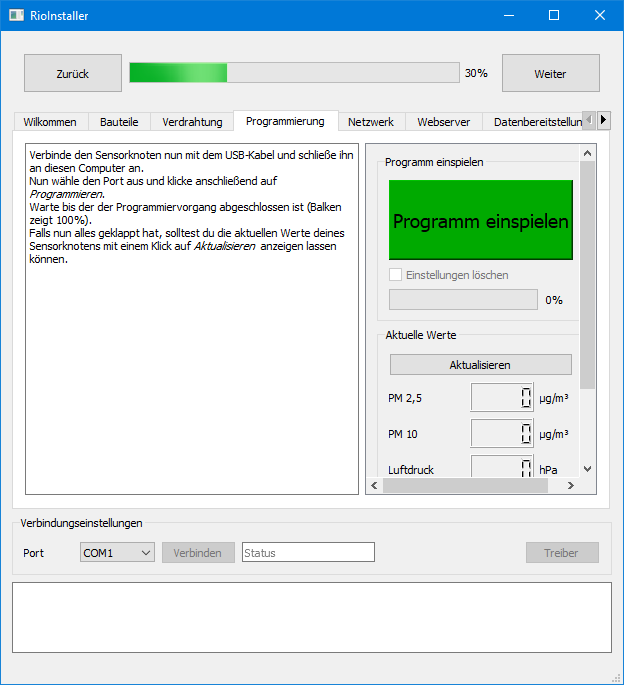
\includegraphics[width=\textwidth]{./ressourcen/Programmierung_neu.png}
	\caption{Reiter: Aufspielen der Firmware}
	\label{fig:skItoolOldFirmware}
\end{figure}

\begin{figure}[H]
	\centering
	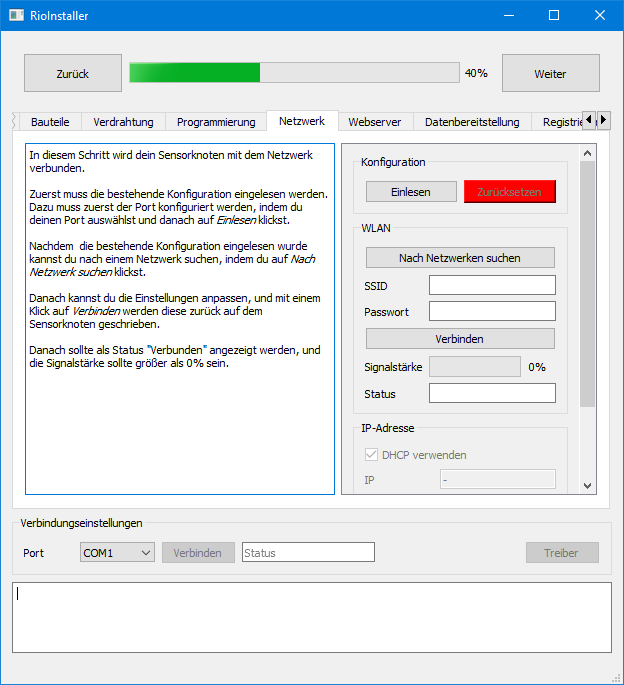
\includegraphics[width=\textwidth]{./ressourcen/Netzwerk_neu.png}
	\caption{Reiter: WLAN Konfiguration}
	\label{fig:skItoolOldWifi}
\end{figure}

Dieses Konfigurationstool wurde beim Schülerinformationstag und bei der Anbringung der Sensorknoten an den jeweiligen Schulen verwendet und erwies sich als ausreichend benuzerfreundlich, um den Sensorknoten in Betrieb zu nehmen.
Das dabei gesammelte Feedback soll daher im weiteren Verlauf des Projektes eingearbeitet werden, um das Konfigurationstool weiter zu verbessern.

\subsection{IoT"=Plattform}
Die im Rahmen des Schülerinformationstages entwickelte prototypische IoT"=Plattform ist die zentrale Schnittstelle zur Annahme und Bereitstellung der gemessenen Messdaten, der bereits im vorherigen Abschnitt beschriebenen Sensorknoten. \\
Für die prototypische Implementierung der IoT"=Plattform wurde die Technologie NodeJS im Zusammenspiel mit einer MongoDB als Datenspeicher eingesetzt.
Diese Entscheidung ist durch die einfache und schnelle Möglichkeiten der Technologien zur Entwicklung eines Prototypen und der bereits vorhanden Erfahrung innerhalb der Projektgruppe zu begründen.
Des Weiteren bietet NodeJS durch die Verwendung von JavaScript eine große Sammlung an bereits vorhanden Lösungen zu ähnlichen Problemen was die Entscheidung nur noch bekräftigt hat. \\
Die Hauptfunktionen der IoT"=Plattform sind dabei die Annahme der Messdaten von authentifizierten Sensorknoten, die Speicherung dieser und der anschließenden Bereitstellung für die Webseite, welche ebenfalls im Rahmen des Schülerinformationstages implementiert wurde.
Um diese Hauptfunktionen zu realisieren wurde ein HTTP"=Server mit spezifischen Endpunkten zur Authentifizierung, Annahme und Bereitstellung der Messdaten implementiert.
Des Weiteren kommt die bereits genannte Datenbank MongoDB zum Einsatz für die dauerhafte Speicherung der Mess- und Nutzerdaten. \\
Zur Authentifizierung an der IoT"=Plattform wird der OAuth2.0 Standard verwendet.
Dieser erlaubt eine sichere und einfache Authentifizierung von Nutzern der IoT"=Plattform, welche im Falle des Schülerinformationstages die Sensorknoten und Webseite sind.
Vom Standard wird der Client Credentials Flow verwendet, welche den Nutzern erlaubt Benutzername und Passwort für ein JSON Web Token auszutauschen, welches zur Bereitstellung von neuen Messdaten oder der Abfrage von Bestehenden verwendet werden kann. \\
Die Schnittstelle zur Annahme von Messdaten ist nur für Sensorknoten verwendbar, was mit Hilfe des übergebenen JSON Web Token überprüft wird.
Der Sensorknoten übermitteln bei der Schnittstelle per HTTP POST ihre aktuelle Position und die gemessenen Messdaten, welche nach einer Validierung in der Datenbank gespeichert werden. \\
Damit die im Schülerinformationstag entwickelte Webseite die vorhanden Messdaten anzeigen kann wurde die Schnittstelle zur Bereitstellung der Messdaten implementiert.
Dabei kann die Webseite über gesonderte Schnittstellen alle Messdaten aller Sensorknoten, alle Messdaten eines speziellen Sensorknoten und alle Messdaten eines speziellen Sensorknoten, welche in einem bestimmten zeitlichen Intervall liegen, abfragen.  

\subsection{Webseite}

Eine weitere wichtige Komponente des Schülerinformationstages ist das Frontend, beziehungsweise die Webseite, mit dem Ziel, die gemessenen Daten live anzeigen zu können.
Das dabei entwickelte Frontend soll weiterhin für die Schulen und Schüler zur Verfügung stehen, damit diese auch nach dem Schülerinformationstag und der Anbringung der Sensoren ihre gemessenen Daten einsehen und ggf. analysieren können.
Um dieses Ziel zu erreichen haben wir uns für eine Webseite mit dem Angular"=Framework entschieden, was zum größten Teil mit den bereits vorhandenen Erfahrungen innerhalb der Projektgruppe zusammenhängt, da mehrere Mitglieder bereits mit diesem Framework gearbeitet haben und die Vorbereitungszeit sehr begrenzt war.
Um den Schülerinnen und Schülern eine ansprechende Darstellung der Werte zu liefern, haben wir uns für eine Visualisierung der Daten als Diagramm, welches durch Highcharts unterstützt wird, entschieden.
Dabei handelt es sich um ein Plugin, welches auf Javascript basiert und das angezeigte Diagramm anhand von verschiedener Datensätze anzeigen kann.
Außerdem wird die Darstellung der HTML"=Elemente durch die Bootstrap"=Bibliothek unterstützt.

\begin{figure}[H]
	\centering
	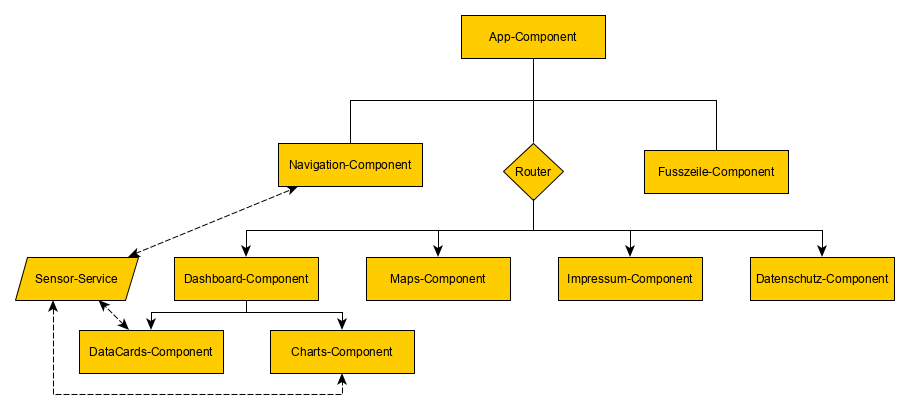
\includegraphics[width=\textwidth]{./ressourcen/schit-aufbau-frontend.png}
	\caption{Grundaufbau der Webseite}
\end{figure}

Die dabei entwickelte Applikation ist aus verschiedenen Komponenten aufgebaut.
Eine Komponente besteht aus einer HTML, einer SCSS und einer Typescript"=Datei.
Der Kern der Komponenten ist die App"=Komponente.
In dieser werden alle anderen Ansichten rein geladen.
Der Navigations- und der Fußzeilenbereich werden durchgehend angezeigt.
Die anderen Komponenten werden durch den Router in der Mitte der Applikation geladen. 

\begin{figure}[h]
	\centering
	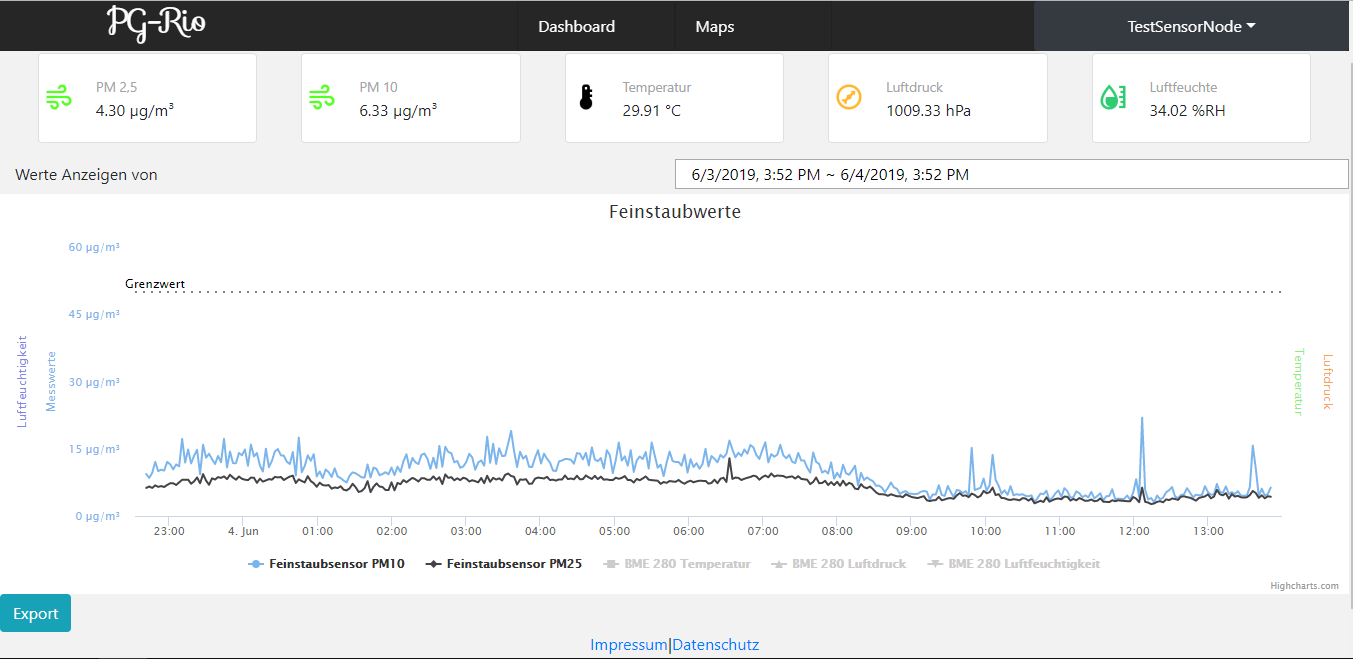
\includegraphics[width=\textwidth]{./ressourcen/schit-dashboard-frontend.png}
	\caption{Dashboard der Webseite}
\end{figure}

Beim ersten Aufrufen der Applikation wird auf die Dashboard"=Komponente weitergeleitet.
Diese bekommt dabei ihre Informationen von dem Sensor"=Service, welcher für die Kommunikation mit der IoT"=Plattform zuständig ist.
Er lädt die Daten von den ausgewählten Sensoren und bereitet sie für die Data"=Cards und das Diagramm auf.
Die Daten werden zu Beginn für den heutigen Tag geladen.
Um die Daten anderer Tage einzusehen, kann durch einen Kalender oberhalb des Charts ein anderer Zeitbereich ausgewählt werden, sodass auch ganze Wochen eingesehen werden können.
Im unteren Bereichs der Chart"=Komponente gibt es eine Möglichkeit, die Daten, die derzeit im Chart angezeigt werden, als CSV"=Datei zu exportieren.
Dabei werden die Sensordaten mit einem Zeitstempel im Unixformat versehen. 

Die Maps"=Komponente ist zur Darstellung der einzelnen Sensoren auf einer Map.
Diese wurden von uns händisch in den Kalender eingetragen.
Außerdem besitzen wir noch ein Impressum und eine Datenschutz"=Seite, um alle relevanten Nutzerdaten bereitzustellen. 


\subsection{Infrastruktur}
Eine weitere zentrale Komponente des Prototyps ist die Infrastruktur.
Um die Messdaten der verteilten Sensorknoten an eine zentrale Stelle senden zu können, diese dort entgegenzunehmen und zu speichern, sind über das Internet erreichbare Server nötig, die diese Dienste bereitstellen.
Des Weiteren muss den Schülerinnen und Schülern der Zugang zu der Webseite zum Anzeigen der gespeicherten Sensordaten über das Internet ermöglicht werden.
Für die Umsetzung dieser Anforderungen hat die Universität Oldenburg Ressourcen zur Nutzung von virtuellen Rechnersystemen (VMs) zur Verfügung gestellt.
In \Fref{fig:schitInfra} ist in einen Netzwerkdiagramm die dafür entwickelte und umgesetzte Infrastruktur für den Schülerinformationstag mit den drei folgenden verwendeten VMs dargestellt:
\begin{itemize}
\item \url{pg-rio-dvlp.Informatik.Uni-Oldenburg.DE} (Entwicklungsserver)
\item \url{pg-rio.Informatik.Uni-Oldenburg.DE} (Produktivserver)
\item \url{pg-rio-strg.Informatik.Uni-Oldenburg.DE} (Fileserver)
\end{itemize}
\newpage
\begin{figure}[H]
	\centering
	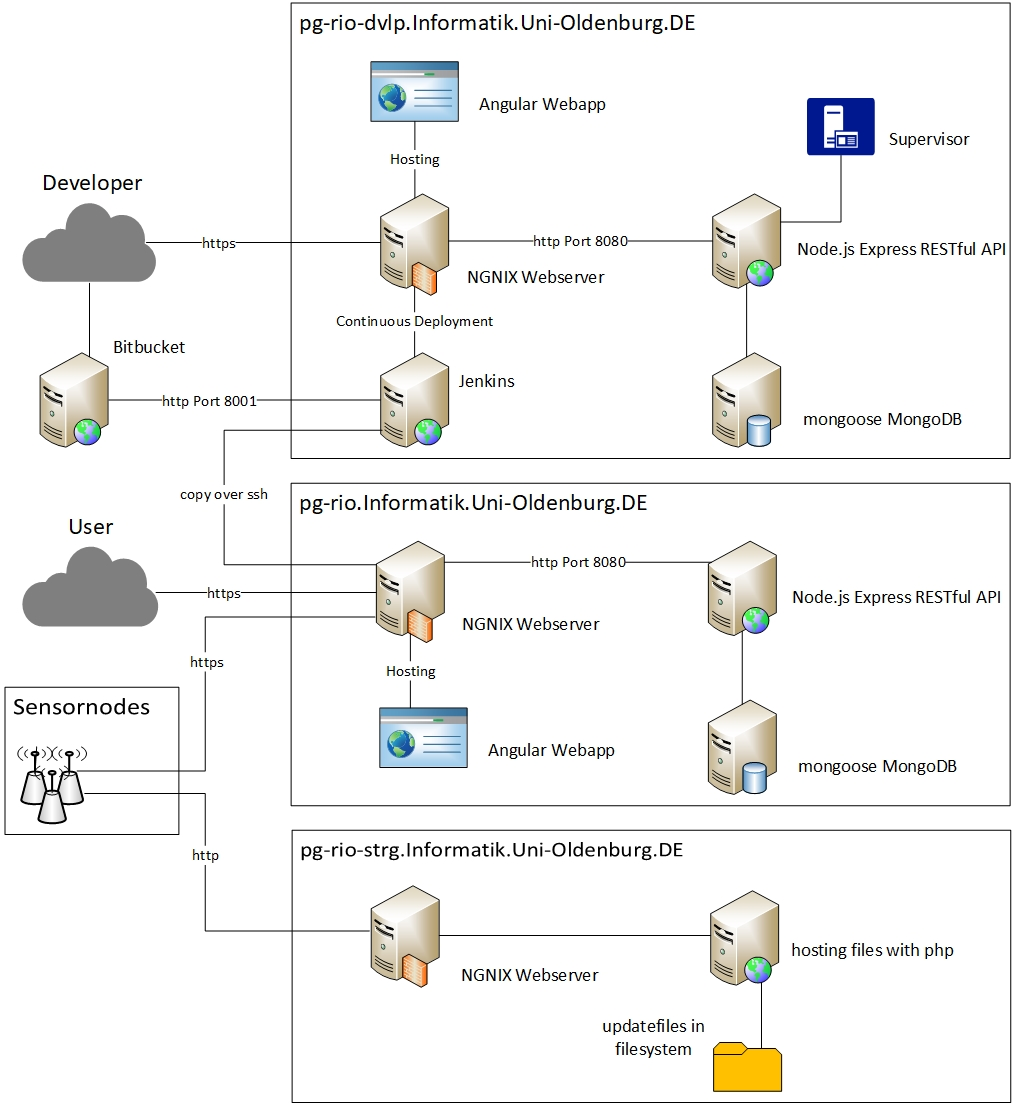
\includegraphics[width=\textwidth]{./ressourcen/SCHIT-Infrastruktur.jpg}
	\caption{Infrastruktur für Schülerinformationstag}
	\label{fig:schitInfra}
\end{figure}
\noindent
Im Folgenden werden die Funktionen der einzelnen Komponenten im Netzwerksdiagramm in \Fref{fig:schitInfra} erläutert:
\begin{itemize}
\item	\textbf{NGINX Webserver}\\
Die Webserver fungieren auf allen drei VMs als Reverse"=Proxy.
Die Aufgabe eines Reverse"=Proxy ist die Zugangskontrolle bei öffentlichen Anfragen über das Internet.
Des Weiteren werden dort die Anfragen zentral protokolliert.
Weitere Aufgaben der Webserver sind die Erreichbarkeit über das Internet mit einer gesicherten Verbindung über https zu ermöglichen, sowie die Webseite über den Entwicklungsserver und den Produktivserver zu veröffentlichen.     
\item	\textbf{Node.js Express RESTful API}\\
Die API ist für die Entgegennahme der Messdaten der Sensorknoten, dem Speichern der Messdaten in eine MongoDB, sowie dem Bereitstellen angefragter Messdaten über die Webseite zuständig.
Auf dem Entwicklungsserver läuft der Dienst in einen Supervisor.
Dieser ermöglicht in der Entwicklungsphase bei auftretenden Fehlern das Protokollieren der Fehlermeldungen, sowie das automatische Neustarten des Dienstes.
\item	\textbf{Jenkins}\\  
Der Jenkins"=Dienst auf dem Entwicklungsserver ermöglicht schnelle Aktualisierungen der Webseite in der Entwicklung.
Dazu ist dieser mit dem Bitbucket"=Dienst der Universität Oldenburg gekoppelt und führt bei Versionsaktualisierungen und Fehlerbehebungsmaßnahmen automatisch Kompiliervorgänge durch und veröffentlicht  aktualisierte Webseitenversionen.
\item	\textbf{Bereitstellung von Updatedateien}\\
Auf dem Fileserver werden Updatedateien für die Sensorknoten über einen php"=Dienst bereitgestellt.     
\end{itemize}

\subsection{Migration}
Am 11. September 2019 wurden die Sensorknoten mit der prototypischen Firmware des Schülerinformationstags auf den Stand der Neuentwicklung migriert und so in das neuentwickelte Produktivsystem eingebunden.
Dazu gibt es eine Migrationsfirmware, die auf dem Updateserver des alten Systems bereitgestellt wurde.
D.h. nur die Sensoren mit der prototypischen Firmware aktualisieren sich auf diese Migrationsfirmware.

Die Migrationsfirmware führt nacheinander folgende Schritte durch:

\begin{enumerate}
	\item Die Konfiguration der alten Firmware wird von \filename{config.json} in \filename{config.old.json} umbenannt.
	\item Die Standardkonfiguration für die neue Firmware wird in die Datei \filename{config.json} geschrieben.
	\item Die Datei \filename{credentials.json} wird durch mehrere Bausteine erzeugt.
	Darin enthalten sind die WLAN"=Zugangsdaten sowie die Zugangsdaten für die IoT"=Plattform aus der alten Konfiguration.
	\item Die mitgelieferte neue Sensorknoten"=Firmware wird in eine Datei auf dem Dateisystem geschrieben.
	\item Das Update wird mit der geschriebenen Update"=Datei durchgeführt.
	\item Die Update"=Datei wird gelöscht und das System neugestartet.
\end{enumerate}

Vorbereitend für die Migration wurden die Zugangsdaten der alten IoT"=Plattform in das neue System übertragen.
Nachdem die Migrationsfirmware hochgeladen wurde, konnten alle betroffenen und erreichbaren Sensorknoten innerhalb von 24 Stunden erfolgreich in das neue System migriert werden.

\section{Fazit}

Zum Abschluss des Berichts zur Teilnahme am Schülerinformationstags soll in Hinblick auf die Erreichung der angestrebten Ziele nun abschließend Bilanz gezogen werden.
Das war zum einen die Erregung von Aufmerksamkeit und zum anderen der Gewinn von Standorten zur Anbringung erster Sensorknoten.
Da im Rahmen des Informationstags nur wenige angebracht werden konnten, muss man in diesem Punkt von einem schlechten Ergebnis sprechen, das den aufgebrachten Aufwand nicht rechtfertigen kann.
Was allerdings die Erregung von Aufmerksamkeit betrifft, so konnten wir zumindest bei unseren Zuhörern und Teilnehmern ein großes Interesse an der verwendeten Technologie sowie der Feinstaub"=Thematik feststellen.
Das widerum gibt Anhaltspunkte für die Planung weiterer Maßnahmen zur Gewinnung von Sensorstandorten in späteren Projektphasen, die es gezielt zu planen gilt.
Denkbar wäre beispielsweise das Angebot weiterer Workshops für z.B. andere Studenten oder umweltbewusste Oldenburger.

Neben den gesetzten Zielen, müssen aber auch die gewonnen Erkenntnisse aus der Entwicklung des Prototyps bewertet werden.
So haben wir einerseits einen Teil Umsetzbarkeit unserer Vision gezeigt, aber auch eine Grundlage zur notwendigen Datenanalyse geschaffen.
Auch bei der Anforderungserhebung konnte der Prototyp helfen, erste Erkenntnisse als Basis zu nutzen.
In der Entwicklung konnten wir bereits vor Beginn der Hauptentwicklungsphase feststellen, wo wir unsere Zusammenarbeit im Team verbessern müssen.
Daher wollen wir ein besonderes Augenmerk darauf setzen, dass wir Wissensinseln vermeiden und die Synchronisation zwischen Teilteams geplant sicherstellen.

Unter Einbezug der erweiterten Erkenntnisse über die gesetzten Ziele hinaus bewerten wir die Teilnahme am Schülerinformationstag daher insgesamt als gelungen und zufriedenstellend.

\let\chapter\oldchapter
\let\section\oldsection\
\let\subsection\oldsubsection
% Hack end.

\section{Meilenstein 1: 10.04.2019 - 24.04.2019}
Der erste Meilenstein 1 in der Entwicklungsphase zeichnet sich dadurch aus, dass in diesem noch keine konkreten funktionalen Anforderungen umgesetzt werden.
Der Fokus des Meilensteins liegt auf der Einarbeitung und dem Aufbau der unterschiedlichen Softwareprojekte.

Diese Phase erweist sich als sehr wichtig für die Projektgruppe, da die einzelnen Komponenten zum Teil in unterschiedlichen Programmiersprachen erstellt werden.
Zudem werden verschiedenste Frameworks genutzt, um die Entwicklungsphase zu erleichtern.
So steht neben dem Projektsetup auch noch viel Recherchearbeit zu möglichen Plugins und Frameworks an, die zwar in der Architektur bereits betrachtet wurden, jedoch bis zu diesem Zeitpunkt noch nicht zum tatsächlichen Einsatz gekommen sind.
Das Ziel ist es, dass mit Abschluss des Meilensteins, die PG=Mitglieder die tatsächliche Umsetzung von funktionalen Anforderungen in Form von User Stories abarbeiten können.
Innerhalb des ersten Meilensteins werden folgende Komponenten als Projekt aufgesetzt: der Sensorknoten, die IoT"=Plattform, der Routing"=Service und die Navigationsapplikation.

Da im ersten Meilenstein fast keine Anforderungen aus Sicht eines Endnutzers erfüllt werden, gibt es hier keine Demo beziehungsweise eine konkrete Präsentation, mit welcher der Meilenstein als abgeschlossen gilt.
Als Ergebnis lässt sich jedoch festhalten, dass alle geplanten Ziele größtenteils erreicht wurden.
Jedoch ist der Aufwand des Aufsetzens der Projekte in den verschiedenen Teilbereichen unterschiedlich Komplex.
Aus diesem Grund konnte in einigen Gruppen auch schon mit der Umsetzung von funktionalen Anforderungen begonnen werden.
Durch die Fertigstellung der Projektsetups kann im folgenden zweiten Meilenstein mit der Umsetzung der Anforderungen begonnen werden.
Dabei muss jedoch berücksichtigt werden, dass neben den oben genannten Komponenten noch weitere Komponenten im Laufe der Entwicklungsphase hinzukommen werden, welche auch wieder eine kurze Einarbeitungszeit benötigen.
Dazu gehören beispielsweise ein Frontend für den Umweltinformationssystem"=Nutzer oder eine Oberfläche zum Verwalten der Sensorknoten.
Diese Einarbeitungszeit wird dann im Refinement der einzelnen User Stories berücksichtigt.
\section{Meilenstein 2: 24.05.2019 - 22.05.2019}
Der zweite Meilenstein hat das Ziel den Main Showcase abzubilden und so gleichzeitig den technischen Durchstich durch alle Komponenten unseres Systems aufzuzeigen.
Das bedeutet, dass die Sensorknoten in der Lage sind, Daten zu messen und an die IoT-Plattform zu senden.
In der IoT-Plattform werden diese Daten aufgenommen und in einer Datenbank abgespeichert.
Um mit den gespeicherten Daten weiterarbeiten zu können, müssen die Daten über einen Service bei der IoT-Plattform abgefragt werden können.
Diese Daten werden dann von dem Routing-Service genutzt, indem sie in der Berechnung einer Route als Gewichtungsfaktor berücksichtigt werden.
So kann letztendlich die Navigationsapplikation über einen Schnittstelle zum Routing-Algorithmus einen Start- und Endpunkt übergeben, aus welchen eine Route erstellt wird, die man über eine weitere Schnittstelle dem Navigationsnutzer bereitstellt.

Das übergeordnete Ziel des Meilensteins ist es also nicht nur, den technischen Durchstich zu erwirken, sondern auch ein Zusammenspiel aller Komponenten untereinander zu schaffen.
Um dies zu ermöglichen ist es notwendig, dass unter den unterschiedlichen Komponenten beziehungsweise Gruppen Schnittstellen implementiert werden, die zuvor in der Architektur festgelegt worden sind.
Um dieses Ziel zu erreichen, ist ein hoher Abstimmungsaufwand erforderlich sowie das Durchführen von Integrationstests, um sicherzustellen, dass die Schnittstellen zwischen den einzelnen Komponenten funktionsfähig sind.


Zusammenfassend zum zweiten Meilenstein lässt sich festhalten, dass nicht alle geplanten Ziele erreicht werden konnten.
Ein Gesamtbild der Ergebnisse zeigt sich in \Fig{bigpicture1}.
In dieser Abbildung werden zu jedem der vier Teilbereiche die vorher gesetzten Ziele aufgelistet.
Zudem wird farblich gekennzeichnet, ob die Ziele vollständig (grün), zum Teil(gelb) oder gar nicht (rot) erreicht wurden.
Dabei muss berücksichtigt werden, dass es sich bei den Zielen nur um die gesetzten Ziele im Meilenstein handelt und nicht um die Gesamtziele im Projekt.

\begin{figure}[!htb]
	\centering
	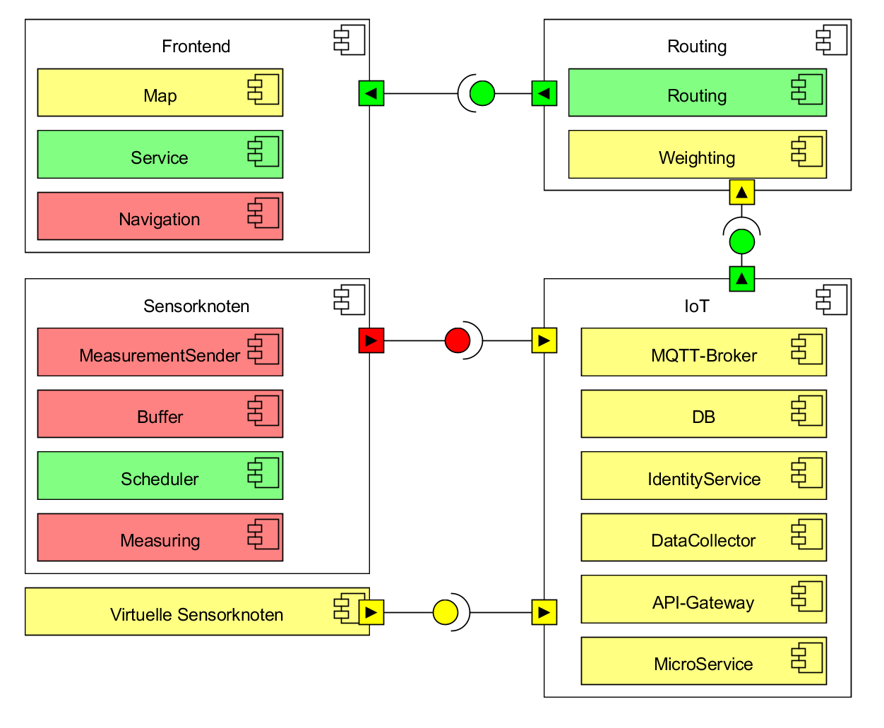
\includegraphics[width=\textwidth]{./ressourcen/bigpicture1.png}
	\caption{Big Picture des ersten Meilensteins}
	\label{fig:bigpicture1}
\end{figure}

In dem Gesamtbild zu den Meilensteinzielen zeigt sich deutlich, dass nicht alle Ziele vollständig erreicht werden konnten.
Unter anderem konnten Themen im Bereich Sensorknoten und Frontend gar nicht erst angegangen werden.
Dies hat verschiedene Gründe: Zum einen ist dieser Meilenstein der erste, bei dem die Projektgruppe mit tatsächlichen Anforderungen aus Sicht eines Nutzers gearbeitet hat.
Das Ergebnis dessen ist, dass viele Aufwände noch falsch eingeschätzt wurden.
Am deutlichsten zeigt sich dies bei der Entwicklung der Firmware für die Sensorknoten und den zu entwickelnden Komponenten der IoT"=Plattform.
So konnte insgesamt kein vollständiger technischer Durchstich des Systems aufgezeigt werden, da zum Beispiel der MeasurementSender der Sensorknoten Firmware noch nicht funktionsfähig war und zudem auch noch keine Schnittstelle zwischen der IoT"=Plattform und dem Sensorknoten zur Verfügung stand.
Dem gegenüber stehen jedoch das nahezu vollständige Erreichen der Ziele in anderen Komponenten wie Routing sowie die Schnittstellen zwischen Routing, IoT und Frontend.
Bei der Bewertung muss jedoch berücksichtigt werden, dass sowohl die Aufwände als auch Einarbeitungszeiten in nahezu allen Gruppen falsch eingeschätzt wurden.
Der Meilenstein hat deutlich aufgezeigt, dass die Gruppeneinteilung sowie die Schätzung der Aufwände an den Jira"=Tickets noch weiter optimiert werden muss.
Der Grund für das nicht"=erreichen der Ziele des zweiten Meilensteins ist nicht darin begründet, dass zu wenig Aufwand von den Mitgliedern der Projektgruppe betrieben wurden, sondern lediglich die Ziele nach einem so kurzen Zeitraum signifikant zu hoch gesteckt wurden.
\section{Meilenstein 3: 22.05.2019 - 03.07.2019}
Der dritte Meilenstein hatte in erster Linie das formulierte Ziel, dass ein Nutzer sich anhand eines selbst gewählten Start- und Endpunktes und unter Berücksichtigung von real gemessenen und simulierten Feinstaubdaten routen lassen kann.
Um dieses Ziel zu erreichen, müssen zudem die offenen Anforderungen aus Meilenstein 2 umgesetzt werden, sodass der vollständige technische Durchstich erreicht wird.
Durch die Sensorknoten sollen Daten gemessen werden, welche in der IoT"=Plattform gespeichert und bereitgestellt werden.
Diese Daten fließen dann in die Berechnung einer Route ein, die anhand eines Start- und Enpunktes vom Navigationsnutzer vorgegeben wird.


Neben dem formulierten Ziel aus Meilenstein 3, werden auch die ersten Anforderungen zum UIS"=Nutzer umgesetzt.
Für die Umsetzung dieser Anforderungen wird zunächst ein neues Projekt aufgesetzt, welches ein eigenes Frontend als Single Page Webseite beinhaltet.
In diesem soll es interessierten Personen ermöglicht werden, die Sensorknoten"=Abdeckung in Oldenburg in einer Karte einzusehen sowie die gemessenen Feinstaubdaten  zu den jeweiligen Sensorknoten.
Um die Daten im Frontend anzeigen zu können, müssen diese zunächst von der IoT"=Plattform abgefragt werden.
Hierfür können zum Teil bereits bestehende Schnittstellen genutzt werden.


Weiterhin ist im Hauptziel des Meilensteins die Rede von simulierten Werten.
In diesem Zusammenhang soll es die Möglichkeit geben, virtuelle Sensorknoten anzulegen und mit den gleichen Informationen (Standort, Id, Höhe...) zu versehen.
Diese Werte sollen dann im Routing"=Service genauso berücksichtigt werden, wie die real gemessenen Daten.
So wird beispielsweise die Möglichkeit geboten, die Abdeckung von Oldenburg mit Feinstaubdaten zu erhöhen.
Dabei muss jedoch berücksichtigt werden, dass im dritten Meilenstein nur eine Strategie umgesetzt wird, in der in einem bestimmten Intervall festgelegte Werte von den virtuellen Sensorknoten gesendet werden.
Im weiteren Verlauf der Projektgruppe sollen weitere Strategien hinzukommen, in denen zum Beispiel die realen Sensorknoten berücksichtigt werden, sodass durch räumliche Interpolation oder andere Verfahren realistische Werte für die virtuellen Sensorknoten erzeugt werden.

\begin{figure}[!htb]
	\centering
	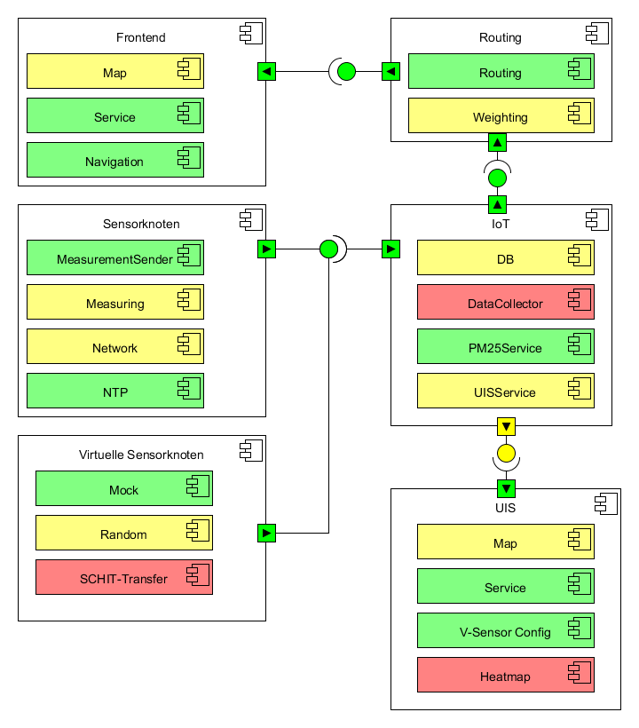
\includegraphics[width=\textwidth]{./ressourcen/bigpicture2.png}
	\caption{Big Picture des dritten Meilensteins}
	\label{fig:bigpicture2}
\end{figure}


Zusammenfassend zeigt sich, dass wieder ein hoher Aufwand an Abstimmungen und Integration zwischen den einzelnen Projekten notwendig ist.
Als Ergebnis des Meilensteins lässt sich festhalten, dass die Schnittstellen zwischen allen System funktionsfähig sind und hier nahezu alle Ziele erreicht worden sind.
Dies zeigt sich auch in \Fig{bigpicture2}.
Jedoch sind auch noch wenige Aufgaben offen, wie das Persistieren von Daten in der Datenbank oder die Integration der Schit"=Daten.
Die in diesem Zusammenhang ausgebrachten Sensorknoten senden momentan noch an eine extra dafür aufgesetzte Plattform.
Um die Daten der Sensorknoten an unser neues System senden zu lassen, sodass die Sensorknoten im Routing berücksichtigt und im UIS"=Frontend angezeigt werden können, muss die Firmware entsprechend geupdated werden.
Aus Zeitgründen und in Hinblick auf die hauptsächlichen Ziele des Meilensteins, wurde die Umsetzung dieser Aufgaben niedriger priorisiert.
Aus diesem Grund wurde eine solche Anforderung im dritten Meilenstein nicht mehr realisiert.
Im Meilenstein ist neben der Umsetzung der offen gebliebenen Anforderungen aus Meilenstein 3 die Möglichkeit des Routens anhand von Temperaturdaten oder anderen vorgesehen.
Dafür muss unter anderem die Sensorknoten"=Firmware erweitert werden, sodass der BME280 die Temperatur, Luftdruck und Luftfeuchte misst, die Werte an die IoT"=Plattform sendet, welche die Werte dann für weitere Services, wie den Routing"=Service bereitstellt.
\section{Meilenstein 4: 03.07.2019 - 07.08.2019}
Der vierte Meilenstein hat das übergeordnete Ziel, das Produktivsystem aufzusetzen und so quasi die erste Version unseres Systems zu veröffentlichen.
Neben dem Aufsetzen des Produktivsystems sollen zudem weitere Anforderungen umgesetzt werden, die vor allem Features für die jeweiligen Endnutzer (also UIS"=Nutzer und Navigationsnutzer) beinhalten.
In Hinblick auf die beschränkte Restdauer der Projektgruppe wurden daher Anforderungen niedriger priorisiert, die zum Beispiel den Umgang mit der IoT"=Plattform erleichtern oder Ähnliches.
Die Priorisierung der noch bis zum Projektende geplanten Features wurde innerhalb der Umsetzung des Meilensteins mit den Stakeholdern abgestimmt.


In der Vorbereitung des Meilensteins werden daher Szenarien geplant, die mit Abschluss des Meilensteins in Form einer Demo gezeigt werden sollen.
Insgesamt gibt es vier verschiedene Szenarien: Das erste Szenario ist bezogen auf den Navigationsnutzer und beginnt damit, dass der Nutzer einen Start- und Endpunkt in der Navigationsapplikation sowie als Fahrzeug ein Auto auswählen kann.
Nach der Planung der Route werden mehrere Routen vorgeschlagen, welche die vorher festgelegten Parameter erfüllen.
Daraufhin soll der Navigationsnutzer in der Lage sein, nicht die erst ausgewählte (beste) Route zu nehmen, sondern eine der alternativen Routen.
Dann soll der Navigationsnutzer die Navigation starten und abbrechen können.
Das zweite Szenario bezieht sich auch auf den Navigationsnutzer und ist ähnlich aufgebaut das erste Szenario.
Der Unterschied besteht darin, dass unterschiedliche Parameter ausgewählt werden, wie beispielsweise als Fahrzeug ein Fahrrad und die Wahl der besten Route.
Zudem soll eine tatsächliche Navigation stattfinden, indem zum jeweiligen Standort des Navigationsnutzer die entsprechende Navigationsanweisung anzeigt und die bereits zurückgelegte Strecke eingefärbt wird.
Weiterhin wird bei der Abweichung von der verfolgten Route auf die Abweichung hingewiesen.
Das dritte Szenario beinhaltet hauptsächlich das Anzeigen von Zeitreihen zu einem bestimmten Sensorknoten.
Um dies zu ermöglichen, müssen zunächst alle Sensorknoten auf einer Karte angezeigt werden und auch auswählbar sein.
In einer Sidebar werden dann detaillierte Informationen zum Sensorknoten angezeigt, sowie die Möglichkeit geboten, Zeitreihen anzuzeigen
 Neben den Zeitreihen soll zudem eine Heatmap in der Karte angezeigt werden, welche die Feinstaubwerte kategorisiert und so die Belastung in Oldenburg sichtbarer macht.
Das vierte und letzte Szenario richtet sich an Projektinteressierte.
Auf der UIS"=Webseite wird erläutert, wie interessierte Personen einen Sensorknoten selber kaufen, aufbauen, einrichten und montieren können, sodass diese Sensorknoten an unsere IoT"=Plattform senden.


Zusammenfassend zu vierten Meilenstein lässt sich festhalten, dass alle funktionalen Anforderungen umgesetzt werden konnten.
Jedoch besteht an einigen Stellen noch Verbesserungsbedarf.
Dies zeigt sich auch in \Fig{bigpicture3}, in welchem wieder die Erreichung der Ziele in den einzelnen Teilprojekten dargestellt ist.
Verbesserungsbedarf besteht zum Beispiel in den Schnittstellen des UIS"=Frontend zur IoT"=Plattform.

\begin{figure}[!htb]
	\centering
	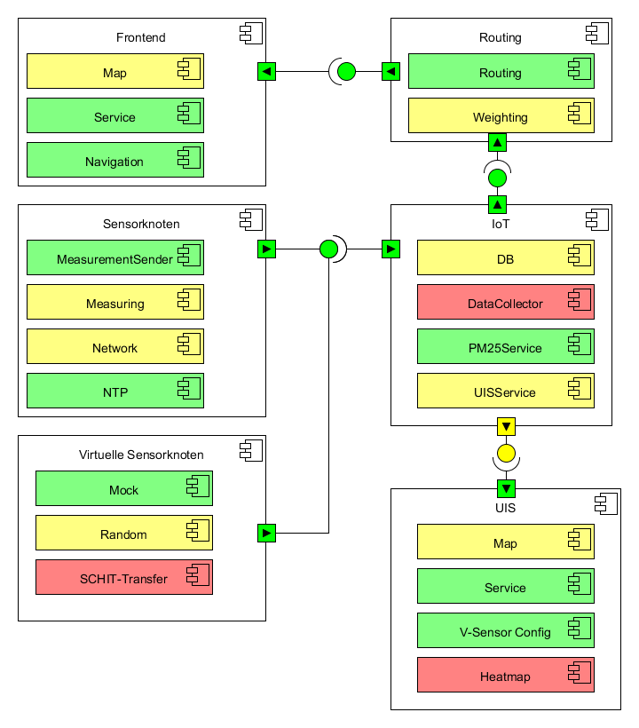
\includegraphics[width=\textwidth]{./ressourcen/bigpicture3.png}
	\caption{Big Picture des vierten Meilensteins}
	\label{fig:bigpicture3}
\end{figure}

So dauert zum Beispiel das Abfragen der Zeitreihendaten eines Sensorknoten bis zu 30 Sekunden.
Neben diesem Umstand gibt es weitere kleinere Fehler, die bis zum Abschluss der Projektgruppe gefixt werden sollten.
Um das System letztendlich robuster zu gestalten, wird in den nächsten Phasen der Projektgruppe der Aspekt des Testens intensiver fokussiert.
Weiterhin sollen diverse weitere Features umgesetzt werden, wie zum Beispiel der Export der Daten eines Sensorknotens.
Zudem soll eine Oberfläche für die Verwaltung von Sensorknoten geschaffen werden und ein Installationstool, welches es Projektinteressierten ermöglicht, die aktuellste Firmware der Projektgruppe auf dem selbst bereitgestellten Sensorknoten zu flashen.
Der dritte Meilenstein zeigt aber insgesamt, dass die Planung und Zusammenarbeit der Projektgruppe immer gezielter und somit auch besser wird.
Dies spiegelt sich insbesondere darin wieder, dass es nur noch weniger Themen gibt, die im Meilenstein gar nicht angegangen worden sind.
Zudem sind die Themen, die in \Fig{bigpicture3} nicht vollständig umgesetzt wurden, oft nahezu fertig und es fehlen noch Kleinigkeiten, wie beispielsweise Unit Tests oder die Entwicklerdokumentation.
\section{Meilenstein 5: 07.08.2019 - 04.09.2019}
Der fünfte Meilenstein ist der letzte der Implementierungsphase.
Mit Abschluss des Meilensteins gilt für die Projektgruppe ein Feature Freeze.
In diesem Meilenstein wird das Ziel verfolgt, das Gesamtsystem mit gezielten Features abzurunden und fertigzustellen.
Durch die bereits bestehenden Schnittstellen zwischen den einzelnen Komponenten konnte vor allem im Frontend der Fokus auf neue Features gelegt werden.
Im UIS"=Frontend sollte insbesondere die Performanz verbessert sowie eine Export"=Funktion für die Sensorknotendaten bereitgestellt werden.
Weiterhin sollen in der Navigationsapplikation die gleiche Heatmap angezeigt werden, die auch im UIS genutzt wird.
Ein weiteres sehr zentrales Feature, welches im vierten Meilenstein implementiert wird, ist das dynamische Routing.
Vom Nutzer kann bei der Routenplanung ein entsprechendes Intervall eingestellt werden, in dem die Umweltparameter überprüft werden, im bei signifikanten Änderungen eine neue Route für den Nutzer zu berechnen.
Zudem sollen weitere Features, wie das Routing nach anderen Umweltparametern und das Anzeigen von Informationen beim Routing im vierten Meilenstein fertiggestellt werden.


Ein weiteres zentrales Feature ist die Sensorknotenverwaltung, die als Single"=Page"=Webseite implementiert wird.
Hier soll es möglich sein, neue Sensorknoten in der IoT"=Plattform anzulegen und verändern zu können.
Neben der Sensorknotenverwaltung werden in der IoT"=Plattform aufbereitete PM25"=Werte bereitgestellt, welche die Luftfeuchte berücksichtigen.
Diese Werte können für jeden Sensorknoten in den Zeitreihen des UIS"=Frontends angezeigt werden.


Im Kontext der Sensorknotenfirmware wird das Installationstool für Sensorknotenbetreiber bereitgestellt, sodass diese den Sensorknoten auf einfache Weise flashen und konfigurieren können.
Außerdem wird die Möglichkeit geschaffen, die Sensorknoten automatisch zu updaten.
Die virtuellen Sensorknoten sollen neben der Mock"=Strategie und der Random"=Strategie zukünftig auch eine Gewichtungsstragie verfolgen können.
In diesem Zusammenhang soll die Möglichkeit geschaffen werden, diverse reale Sensorknoten anzugeben, die in der Berechnung des virtuellen PM25"=Wertes berücksichtigt werden, sodass ein möglichst realistischer Wert für den virtuellen Sensorknoten erzeugt wird.

\begin{figure}[!htb]
	\centering
	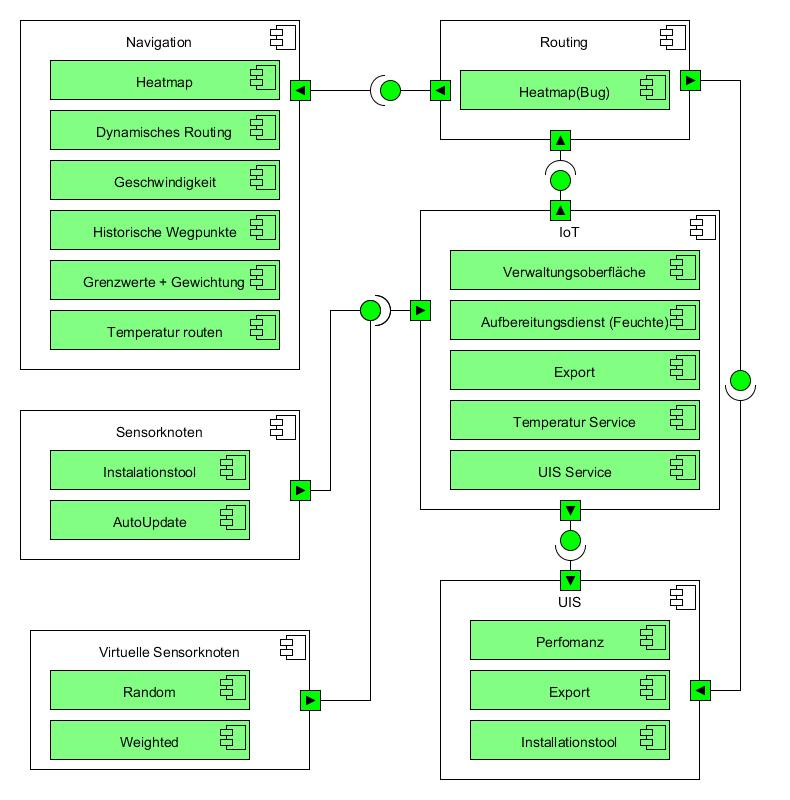
\includegraphics[width=\textwidth]{./ressourcen/bigpicture4.png}
	\caption{Big Picture des fünften Meilensteins}
	\label{fig:bigpicture4}
\end{figure}

In \Fig{bigpicture4} zeigt sich abschließend, dass alle geplanten Ziele für den fünften Meilenstein erreicht wurden.
Durch die Fertigstellung der Schnittstellen zwischen den einzelnen System wird das Arbeiten an Features weniger Komplex.
Hinzu kommt die zunehmende Erfahrung der Projektgruppe in ihren Bereichen, sodass die Umsetzung einer funktionalen Anforderung zum Teil wesentlich schneller voran geht, als am Anfang der Implementierungsphase.
Abschließend wird mit dem fünften Meilenstein das System erfolgreich abgerundet.
Durch das Erreichen aller Ziele, kann in der letzten Phase des Projektes der Fokus auf die Qualität des Systems gelegt werden, welche schon während des Projektes durch Dinge wie die Definition of Done und Ähnliches berücksichtigt wurde.
Dem gegenüber stehen Dinge wie die User Tests, um beispielsweise Feedback einzuholen.
Daher wird für den letzten Monat der Fokus der Projektgruppe auf das Testen, Bugfixing und Dokumentieren gelegt.

